\documentclass[letterpaper]{article}
%\usepackage{times}
%\usepackage{helvet}
%\usepackage{courier}
\usepackage{cite}
\usepackage{amsmath}
\usepackage{amsthm}
\usepackage{graphicx}
\usepackage{fancyhdr}
\usepackage[bottom]{footmisc}
\usepackage{amssymb}
\usepackage{enumerate}
\usepackage{mathtools}
\usepackage{array}
\usepackage{color}
% algorithms
\usepackage{algorithm}
\usepackage[noend]{algpseudocode}
\usepackage{enumitem}
\usepackage[table]{xcolor}
\usepackage{diagbox}
%===================================
% margins
\usepackage{geometry}
%\geometry{
%	letterpaper,
%	right=20mm,
%	left=20mm,
%	top=10mm,
%	bottom=20mm
%}
\usepackage[pdftex,
 pdfauthor=Soheil Gharatappeh,
 pdftitle={Predicting Death In Game of Thrones},
 pdfsubject={Sample document with blind text},
 pdfkeywords={hyperref, PDF meta information},
 pdfproducer=TeXShop,
 pdfcreator=pdflatex]{hyperref}

%============ FUNCTIONS =============
\newcommand{\valatrisk}[2]{\operatorname{VaR}_{#1}(#2)}
\newcommand{\cvalatrisk}[2]{\operatorname{CVaR}_{#1}(#2)}
\newcommand{\norm}[2]{{\Vert{#1}\Vert}_{#2}}

\newenvironment{mprog}{\begin{array}{>{\displaystyle}l>{\displaystyle}l>{\displaystyle}l}}{\end{array}}
\newcommand{\cs}{\\[1ex] & }
\newcommand{\stc}{\\[1ex] \mbox{s.t.} &}
\newcommand{\minimize}[1]{\min_{#1} &}
\newcommand{\maximize}[1]{\max_{#1} &}

\newcommand{\tr}{^{\mathsf{T}}}
\newcommand{\zero}{\mathbf{0}}
\newcommand{\st}{\quad\text{s.t.}\quad}
%===================================

\newcommand{\eye}{\mathbf{I}}
\newcommand{\one}{\mathbf{1}}
\newcommand{\marek}[1]{\textcolor{red}{[#1]}}

\frenchspacing
\setlength{\pdfpagewidth}{8.5in}
\setlength{\pdfpageheight}{11in}
\pdfinfo{
/Title (Predicting Death In Game of Thrones)
/Author (Soheil Gharatappeh)}
% \setcounter{secnumdepth}{0}  

\title{Predicting Death In Game of Thrones}
\author{Soheil Gharatappeh}

\begin{document}
\maketitle
	
	
% \begin{abstract}
% \begin{quote}

% \end{quote}
% \end{abstract}

\section{Introduction}
These days Machine Learning tools are being widely used to predict different phenomenas. From the stock market, to autonomous cars, researchers are interested to have their prediction on all aspects of life. Recently, the movie Game of Thrones has gained a huge popularity, and everyone was wondering \textit{which of the characters can make it to the end?}. This could be a great subject for a research project in Data Science realm. There are various resources of information, from structured wikis to un-structured text such as the books of this legend. We can base our prediction on information that is coming from all of these resources. However, using the right information helps to put all pieces of this puzzle together.


One rich and valuable piece of information we have access to is a data set obtained by the fan's community. This data set contains various information, from the date of birth, to the allegiances, nobility, gender, etc., and can be used to train different machine learning methods, in order to find out what aspects of the information is the most influential in the chance of death for each character.


For the next phase in the project, we would like to omit the data set, and work only with the wiki and un-structured text of the books. This means the project will shift from a purely machine learning project, towards a more realistic practical data science one, where we need to obtain the information we need, clean it, filter it, and then use that information as a single feature for the machine learning algorithm. Obtaining information from un-structured text is very hard, due to the noisy and nonlinear nature of natural language. 


In order to tackle this issue, we can use knowledge bases. A knowledge base is a big set of triple entities (two names connected with a relation), obtained from a structured text such as wiki, and contains rich information about the world's entities, their meanings, and relationships. Knowledge bases give structure to the raw and noisy data obtained from the web, and makes them usable for a machine. A crucial part of this process is entity linking, where a named entity is linked to the knowledge base.


This work is heavily based on the idea of entity linking and knowledge graphs. In the following sections, we first introduce entity linking and review a few related works in this area. Then, we explain our approach to the problem of using entity linking in order to predict the chance of death for a GoT character, and at the end, we evaluate our work using different measures.

\section{Background}

Knowledge sharing platforms such as Wikipedia, play an important role in creating machine-readable knowledge bases. Knowledge bases contain rich information about the world's entity, and their relationships. Using KB's, one can extract useful information from the raw and noisy data in a text. Entity linking is a key element of this process, where a named entity is linked to the knowledge base.

The entity linking is a challenging task. Name variations, aliases, abbreviations, alternate spellings result in entity ambiguity. The task is to find a map from between a set of pre-identified textual entity mentions m into their corresponding entity in the knowledge base. There, also, might be some entities in the text with no entity record in the knowledge base (unlinkables or NILs).

The process starts with name entity recognition, where the boundaries of the entity is identified. There are three steps in the task of entity linking; candidate entity generation, candidate entity ranking, and unlinkable mention prediction. In the first step, a relevant subset of entities are retrieved from the knowledge base. Then, we need to rank them in the next step, so that we know which node in the knowledge base is more relevant to our entity and which one is less relevant. And, at the end, we need to have a strategy to deal with unlinkables \cite{entity}.


In order to evaluate each of these algorithms, a few metrics have been introduced in \cite{entity}, such as precision, recall, accuracy, and F1-score. Also, some data sets are published in \cite{entity} in order to be used as the ground truth for this field. Going through the list of all available data sets is out of the scope of this writing.

 
In another related work, Cheng et at. introduced Relational Inference for Wikification \cite{cheng-2013}, where they are trying to disambiguate entities in a text by identifying the context of it, and relating an entity to the most relevant Wikipedia page. The idea is to use the relational structure of the text in order to generate more relevant title candidates, rank them better and deal with unlinkables more efficiently. They form an Integer Linear Program using the document and the knowledge base consist of triples, and solve it to find the best assignment for each title-surface set (where surface is an entity mention). This approach is evaluated in comparison to other Wikification systems such as Milne and Witten (M\&W), and Ratinov et al. (R\&R) by using data sets from GLOW system, a work by Ratinov et al. and evaluating it with Bag of Titles (BOT) F1 measure. The results suggest a good level of improvement over all 4 different data sets, in comparison with M\&W and R\&R. They also compared their approach to top 3 TAC 2011 systems, where they used $B^3$ and Micro-Average as the evaluation metric. Their system performed comparatively similar to the top 3.


Also, in \cite{tagme}, Ferragina et al. talk about adding Wikipedia links to the respective mentions of entities in a text. The contribution of this method is its applicability to short or poorly composed texts, such as tweets, snippets of search engines, etc. The idea is to use Wikipedia anchor texts as spots and pages that are linked to them as a possible meaning for each entity. The ambiguity is solved by using a fast and effective scoring function, which exploits the sparseness of the anchors in a short text. One important phase in disambiguation is prunning un-meaningful anchors by using the link probability and coherence of a candidate annotation. This approach is evaluated in comparison Milne \& Witten method on three different data sets, the first one is derived manually, and the second and the third is from Wikipedia. They evaluating their method with F measure, precision and recall. The results show that tagme outperformed in short texts, and have a good comparative performance on long texts in compared with Milne \& Witten method.


In \cite{dbpedia}, Mendes et at. explain their approach to automating the process of text document annotation with DBpedia URIs. The goal is to find and disambiguate DBpedia mentions automatically and adaptively, for the needs of each user, specifically. The idea is, to recognize the entity in a sentence, first. Then,to map the entity to a selection of candidates from DBpedia. Next, using the context around the entity, the disambiguation stage is proceed. And, at the end, we let the user to customize the resulted annotation for his need through the configuration parameters. They evaluated their disambiguation strategy on some unseen DBpedia resource mentions from Wikipedia. They used accuracy for evaluating their system, and it suggests a good upgrade in compared to all baseline methods. But, unfortunately, they didn't provide any accuracy results for other publicly available approaches, and they only compared their algorithm with those methods in terms of precision-recall paradigm. They also tested their system on a set of manually annotated news article, and compared their annotation with other publicly available annotation systems. They evaluate their algorithm using F1 measure and compared it to other methods. But, as the result suggested, they could not outperform the wiki machine. But, they did better than the others in terms of F1 score.


\section{Approaches} \label{sec:approach}

In this section, the approaches for tackling the problem of predicting the death of a GoT character are explained. 
% Preprocessing
There are multiple sources available for extracting information to facilitate the prediction procedure. The main two resources were the five books of Game of Thrones, and the fan-based Wiki website that is crawled and available for us. The Wiki is more structured and organized, and can potentially be used as a knowledge base. On the other hand, the books are unstructured and contain highly noisy information. It is usually very hard to extract information from an unstructured text. But, we are trying to tackle this issue using various tools in machine learning and natural language processing.

\subsection{Preprocessing}
The majority of the features are coming from the books. So, it is very crucial to make the text as clean as possible. This will allow the algorithms to work better, and reach to the level of accuracy that they are designed for. The text books are downloaded from the official Kaggle competition, and have been run through some cleaning phases to remove non-ASCI characters. They are also tokenized, split into sentences, lowercased, and lemmatized using python NLP package. The stop words are also dropped from the texts. 

Next we are going to explain the features that are extracted from the book or the knowledge graph, and the intuition behind them.


 % in this project, we are focused on extracting specific relation
% One of the main ideas were to first train a perfect classifier using the data set, and then discard the features that are read from the prepared data set, and extract those features purely from the books. Although the idea seemed appealing and sound at the beginning, it had a big flaw, and that was; extracting features from an unstructured text is a drastically hard task, if not even impossible.

% This is where having a knowledge base, and doing entity linking over it can be helpful. Using a knowledge base (that is obtained, for example, from the GoT's Wiki), we can employ entity linking in order to disambiguate entities. Entity linking can be helpful in constructing a big feature vector for each entity (each attribute in the Wiki can be served as a feature), which can later on be used to train a classifier. The more accurate entity linker we use, the better result we get from the classifier.



% \subsection{Entity Linking}


% However, having a complete knowledge base is essential in the process of entity linking. It is usually the case that because of having multiple entity in the knowledge base corresponding to the surface, we need to rank the entities so that we can retrieve the most relevant entity to the user. But, unfortunately, that is not the case in here. There is a limited number of wiki pages for each character, with a very limited information. Only 263 of characters of the data set have a corresponding node in the knowledge base. Therefore, I did not include the entity linker features into the set of features.


\subsection{Features}
It is very important to determine which features in the data set are the most useful ones. Factoring out the less informative feature eliminates noisy data and helps the classifier to gain a better accuracy, reducing the chance of overfitting, to obtain a better generalization from the data. The problem of finding the best features of the data set is heavily tied with our ability to extract accurate features from the knowledge base and the book. For instance, one can come up with a set of features, with a high accuracy. But, if extracting those features from the text and the wiki is not feasible, then we have to eliminate them.


Based on various experiments, we figured some features are more important than the others, and in the following we are going to explain a set of features that are found to be more useful in training the classifiers
% \begin{enumerate}
% 	\item Mention counts
% 	\item Gender
% 	\item Proximity to deathly words
% 	\item Last n mentions
% 	\item Graph of connected characters
% \end{enumerate}

% Now, we explain the features we used, and what is the intuition behind choosing them and how we think they help in predicting if a character is dead or not.

\subsubsection{Mention Counts}
The number of times a character has appeared in the book is an important measure that shows how crucial was the character in the story. This feature can imply how a character plays a key role, and if it does, how this type of characters are at the risk of dying in this story. In addition, the number of times that a character appears in each of the five books can also be important, as it can be an indicator of when a character has stopped being referred to, which can be translated into the death of a character.

The total number of times that a character has appeared with full name in the text books is used in here. We also have a 5-column feature set, where we split the name mentions into book. 

One of the biggest issues with only string matching when finding mention features, is referring to a name by his/her nickname, or only referring by the corresponding pronoun. This is ambiguous. Especially in a long story such as GoT, the ambiguity caused by the nature of language makes it very hard for a machine to understand which character is being mentioned in which part of the story. In order to solve this, we have to use \textit{Coreference Resolution} algorithms. We do not address this problem in here, and simply use the full name matching criteria to count a mention.

\subsubsection{Gender}
Gender is another contributing factor in the death of a GoT character. Statistics showed that in the land of GoT, it's more likely to be dead when you are a man than when you are a woman. Therefore, we use frequency of pronouns and the closest pronoun to create two sets of features, called gender feature.

To make this feature, we considered the sentence that a character is mentioned in, and we concatenate this sentence to the next sentence. Then we count the number of pronouns that are found in this large sentence and form the frequency of pronoun feature. We also find the nearest pronoun to the name mention, and assign that pronoun to the character. Since each character is mentioned multiple times throughout the books, we repeat this process multiple times and take votes among different sentences. We used five distinctive mentions of a character in our experiments to take votes.


\subsubsection{Proximity to Deathly Word}
It is common sense that if a character appears around words that imply death is more likely to die. The character is probably a warrior, or very close to the center of tensions. That is why we think occurrence of a character with a deathly word in the same sentence can make a good feature. 

Counting the number of occurrences of a character around deathly words is one measure that we employed to extract a feature. However, it is not the most accurate one. Tf-idf is another measure of closeness in the field of information retrieval, which has shown more promising results. To obtain the proximity of a character to deathly words using tf-idf, we first find the sentences that a character appeared in the book, and create a document out of these sentences. Then the tf-idf score of this document is calculated against a sentence containing all of the deathly words (a hand-crafted list of words prepared for this matter which contains words like stab, kill, die, etc.) and the character's name.


Inspired by the proximity to deathly words features, we created another set of features called \textit{Last n Mentions}. This features contain the number of times a deathly word appeared in the last $n$ mentions of a character. The intuition behind adding this feature was, it is usually the case that when a character stopped being referred to, is the end of the life of the character, especially if the final words contain words revolving around death.

We simply used the deathly word count to create these features, and tried different $n$s, and picked 1 and 5 that showed better performances.


\subsubsection{Graphs}
The relation between characters, being brother, sister, enemy, friend, ally, etc. with other characters is another key factor in the chance of dying in this story. This network representation of characters help us to extract important features from the graph of characters such as betweenness centrality, closeness centrality, degree centrality, Page Rank (which characters are most referred to).

The graph, however, can be created in different ways. Two strategies that we used in this project was as follows:
\begin{enumerate}[label=\alph*.]
	\item Characters are related if they appear in the same sentence
	\item Characters are related if they appear in the same page in the knowledge base
\end{enumerate}


\subsection{Gender Prediction}

Due to the importance of gender among other features in this project, we try to apply more sophisticated tools on the information that is already extracted, and determine the gender with a higher accuracy. So far, we extracted two gender-based features from the text books to use them in the task of predicting death.

However, we can do more with those two gender-based features. We can train an independent classifier using the features to predict gender. We choose a logistic regression, SVC and a decision tree classifier to do that.



% Due to the natural ability of English Language in specifying the gender of a noun phrase in a sentence, there seems to be a possibility for predicting the gender of a character. This gender predictor is based on the use of pronouns in the sentences surrounding a character name, as explained before.

% First, we use a pronoun counter to make the decision about the gender of character. We count the number of pronouns in the sentence that a name has occurred, plus the sentence that comes immediately after. The gender is determined by the dominant pronoun. 

% Second, we apply closeness measure to predict the gender. The gender of the closest pronoun is assigned to each corresponding noun. 

% However, in here, we used the information we extract from the rule-based classifiers as a set of features in order to train a few classifiers. Classification methods that has shown to be promising on this project, such as decision tree and KNN, as well as a logistic regression classifier is selected to be run on this data set. 


% out that features such as the gender, the mention frequency, mention of the name in different sections of the book and how the mention count distributed among different books, and proximity of the character's name in the book to some deathly words are the most useful features. Therefore, we employ various tools to obtain a prediction from the above-mentioned features. 




% We also create different types of knowledge graphs using the knowledge base, by extracting different aspects of each character. For instance, in case of the gender predictor, we can use the information we have in a the wiki page of the character to extract the gender. We can use the idea of pronoun count in the wiki to predict the gender. Also, other informations from the knowledge base, such as the relation between characters can be used to create a graph and measure the centrality of each character, and the closeness of a character to more important figures.




% approaches
%     entity linking and other methods,
%     gender classifier
%     preprocessing
%     features (can include the entity linking features in here)
%     ML/how to combine them



\section{Evaluation}

In this section, we evaluate our work in terms of F1-score metric. The data set of 918 names is downloaded from Kaggle's official competition webpage, and is divided into training and test sets. The death of these character names are supposed to be predicted. The rows in odd indices are used as the training set and even rows are used for testing. 

In order to measure the randomness in the result we obtain, we create 10 random subsets of 200 names. Then, we calculate the evaluation metric for each subset of names independently, and take average over all of experiments.


Figure \ref{fig:f1} shows the performance of different classifiers on this data set. As shown in this figure, decision tree was able to capture the trends in the data better, and predict more accurately. In addition, by looking at figure \ref{fig:f1} one can immediately conclude that linear models didn't work well on this data set at all. This shows there is no linear relation between the features and the response.

% The following plot is F1-score of various classifiers using the same set of features.

% As one can see in figure \ref{fig:f1}, decision tree has the best score, with the f1-score of $0.401$. One thing that is obvious from figure \ref{fig:f1} is . They were not able to generalize the data.

% It is worth mentioning that in the process of adding more features to the system, the f1-score for the best-performing method has changed from $0.6349$ with only count features to $0.6364$ by adding the gender, and to $0.6383$ when adding the deathly word proximity features.

\begin{figure}
	\centering
	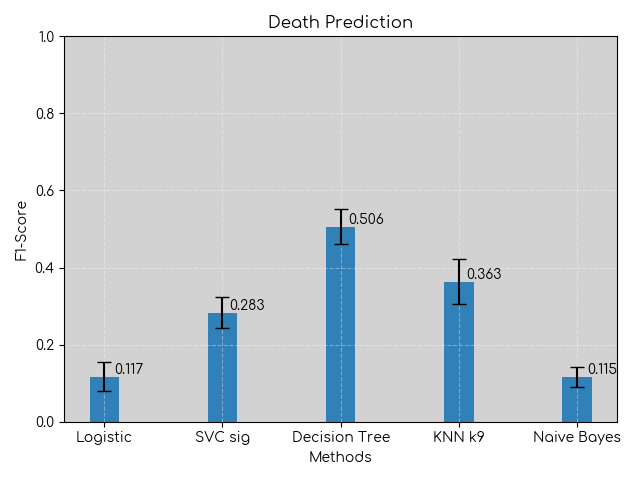
\includegraphics[scale=.60]{death_fscore_error.png} %../../output/
	\caption{F1-score of various classifiers on a set of features completely obtained from the text. The standard error for classifiers from left to right are $0.04, 0.04, 0.05, 0.06, 0.03$ respectively}
	\label{fig:f1}
\end{figure}

\subsection{Gender Predictor}

In another experiment, the rule-based gender classifiers explained in section \nameref{sec:approach} trained and tested using the same data set as the previous experiment. In here, at first a frequency based model is tested. This model could obtain a f1-score of $0.902$. Then, the closest pronoun policy obtained f1-score of $0.623$. After running these rule-based classifiers, we treated them as a set of features and used them to train some standard classifiers, such as SVC and decision tree. The result of this experiment is shown in figure \ref{fig:gender}.

\begin{figure}
	\centering
	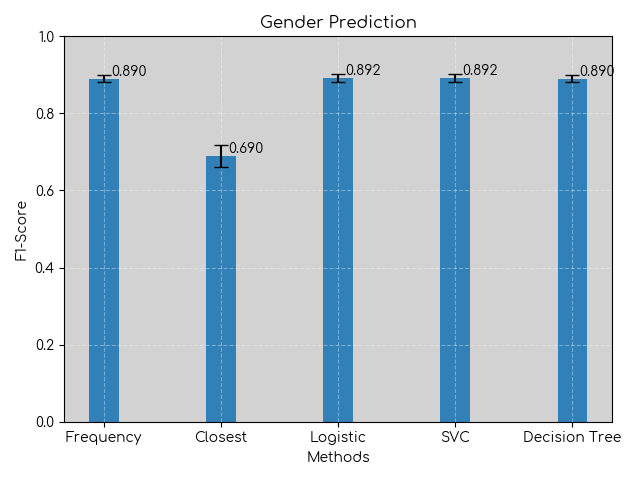
\includegraphics[scale=.60]{gender_fscore_error.png}
	\caption{F1-score of gender classifier. The first two bars are related to the rule-base predictor, and bar 3-5 are f1-score of different classifiers using those rule-base feature for training.}
	\label{fig:gender}
\end{figure}


Interestingly, classifiers could not obtain a f1-score higher than the frequency based method. And, also the type of classifier did not make a difference in this case. We can only conclude that the features are highly correlated, and adding the second feature did not improve the performance of the classifier. In table \ref{tab:gender} we can see the content of confusion matrix for the rule based classifiers and standard classifiers. 


\begin{table}\label{tab:gender}
\centering
\begin{tabular}{ |c|c|c|c|c| } 
 \hline
 Name & TN & FN & FP & TP \\
 \hline
 Frequency &  0 & 80 & 2 & 376 \\
 Closeness & 41 & 39 & 161 & 217 \\
 Logistic &  0 & 80 & 2 & 376 \\
 SVC &  0 & 80 & 0 & 378 \\
 Decision Tree &  0 & 80 & 2 & 376 \\

 \hline
\end{tabular}
\caption{In this assessment, female is considered to be false. So, TN is the number of females characters that the classifier predicted correctly, TP is the number of male characters that the classifier predicted correctly, etc.}
\end{table}



\subsection{Ablation Test}
After adding a lot of features to the training set of a classifier, the next step is to figure out were those features actually useful in the final prediction, or they only add noisy data to the system and cause it to overfit. A great way to show how good and useful was a set of feature is to do ablation test.

In ablation test, we remove a feature from the whole data set and calculate the evaluation metric (f1-score in our case). If f1-score of the newly created data set is more than the original data set, the feature that we just removed was bad and useless. So, we can remove it from the system to increase the accuracy of prediction. On the other hand, if the f1-score of the newly created data set decreases, it shows that we actually removed a useful feature.

\begin{figure}
	\centering
	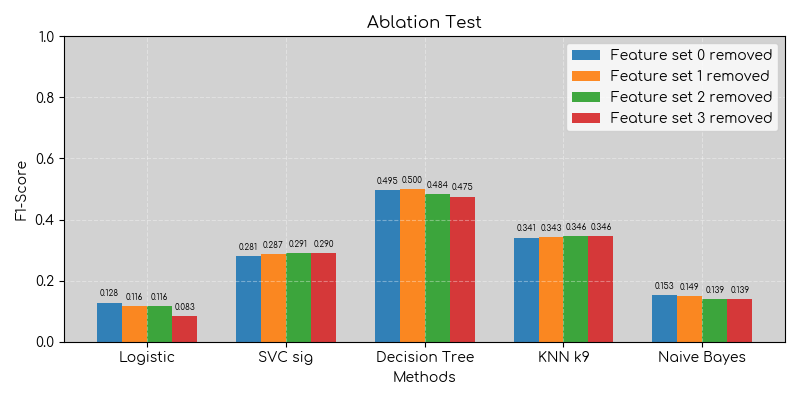
\includegraphics[scale=.70]{ablation.png}
	\caption{Ablation test across various classifiers. Set 1 to 4 are Mention  Counts, Gender, Proximity to Deathly Words, and Graphs.}
	\label{fig:ablation}
\end{figure}

One conclusion that can be drawn from figure \ref{fig:ablation} is that the first set of features, which are mention counts, are highly linearly correlated to the response. When removed from the data set, logistic regression loses its ability to predict accurately, but, SVC actually benefits from not having it. Note that SVC with sigmoid kernel is a nonlinear model, and is not able to capture a linear relation well.

Another conclusion is that decision tree has performed better in general in compared to all other methods.

And, last but not least, there is no evidence that removing a set of feature could increase the f1-score in any meaningful way. This, in other words, means adding each feature has contributed to the improvement of f1-score. So, we keep all of the features in the data set.

\subsection{Best Subset Selection}
We can extend the idea of ablation test to what is called Backward Best Subset Selection. In backward best subset selection the classifier starts with a full set of features, and in each step a feature is removed and the evaluation measure is computed. Next, the feature corresponding to the highest f1-score is removed from the feature set, since removing that feature leads to an improvement in f1-score. This procedure continues until removing a feature does not lead to an improvement. However, due to the heuristic nature of the algorithm it only gives a set of features that locally maximize the f1-score. This means there might be a better subset of feature set that result in a global f1-score maximization. 

In this project, however, due to the randomness of the best-performing algorithm, which is decision tree, we obtain different results across runs. And also, the difference between f1-scores of the feature sets that are removed in each step is very low, that makes the comparison between them meaningless. Table \ref{tab:best_sub} however is one of the results that we obtained running Backward Best Subset Selection. In this table, 8 steps of the algorithm to remove the subset that is associated with highest f1-score is shown. 



\begin{table} \label{tab:best_sub}
\centering
\begin{tabular}{ |c|c|c|c|c|c|c|c|c|c| } 
 \hline
 \diagbox{Step}{Set}  & 1 & 2 & 3 & 4 & 5 & 6 & 7 & 8 & removed \\
 \hline
 1 & 0.476 & 0.479 & 0.491 & 0.494 & 0.473 & \cellcolor{green!25} 0.497 & 0.490 & 0.494 & - \\
 \hline

 2 & 0.473 & \cellcolor{green!25} 0.498 & 0.468 & 0.485 & 0.492 &   -   & 0.482 & 0.498 & 6 \\
 \hline

 3 & \cellcolor{green!25} 0.501  &   -   & 0.475 & 0.486 & 0.501 &   -   & 0.484 & 0.479 & 2 \\
 \hline

 4 &    -   &   -   & 0.482 & 0.473 &\cellcolor{green!25} 0.509 &   -   & 0.476 & 0.4905 & 1 \\ 
 \hline

 5 &    -   &   -   & 0.479 & \cellcolor{green!25}0.498 &   -   &   -   & 0.496 & 0.470 & 5\\ 
 \hline
 
 6 &    -   &   -   & 0.476 &   -    &   -   &   -   & 0.486 & \cellcolor{green!25}0.5 & 4 \\ 
 \hline

 7 &    -   &   -   & \cellcolor{green!25}0.503 &   -    &   -   &   -   & 0.492 &  -   & 8 \\
 \hline
 
 8 &    -   &   -   &   -   &   -    &   -   &   -   &  0.486 &  -  & 3\\

 \hline
\end{tabular}
\caption{The result for Best Subset Selection. The subsets are total counts, counts per book, gender, proximity to deathly word, tf-idf of proximity to deathly word, last 1 mention, last 5 mentions and graph.}
\end{table}

% [{0: [0.4764890282131662], 1: [0.4797507788161993], 2: [0.49079754601226994], 3: [0.49382716049382713], 4: [0.4735202492211838], 5: [0.49693251533742333], 6: [0.4906832298136646], 7: [0.49375]}, 

% {0: [0.47318611987381703], 1: [0.49844236760124616], 2: [0.4683544303797468], 3: [0.48466257668711654], 4: [0.4923076923076923], 6: [0.4829721362229102], 7: [0.49844236760124616]},

%  {0: [0.5015479876160991], 2: [0.47500000000000003], 3: [0.48598130841121495], 4: [0.5015479876160991], 6: [0.4842767295597484], 7: [0.4794952681388013]},

%   {2: [0.4825396825396826], 3: [0.47318611987381703], 4: [0.5092024539877301], 6: [0.4764890282131662], 7: [0.49056603773584906]}, 

%   {2: [0.4794952681388013], 3: [0.49844236760124616], 6: [0.4968553459119497], 7: [0.47021943573667707]}, 

%   {2: [0.4764890282131662], 6: [0.48598130841121495], 7: [0.5]},

%    {2: [0.5031055900621119], 6: [0.4921135646687697]}, 

%    {6: [0.4861538461538461]}]
% [5, 1, 0, 4, 3, 7, 2, 6]
% [0.49693251533742333, 0.49844236760124616, 0.5015479876160991, 0.5092024539877301, 0.49844236760124616, 0.5, 0.5031055900621119, 0.4861538461538461]

% [0.00982966 0.02929984 0.01009634 0.01009634 0.00982966]

 % Step &  \\

%  0.486 & 
% [5, 1, 0, 4, 3, 7, 2, 6]
% [0.49693251533742333, 0.49844236760124616, 0.5015479876160991, 0.5092024539877301, 0.49844236760124616, 0.5, 0.5031055900621119, 0.4861538461538461]

% [0.00982966 0.02929984 0.01009634 0.01009634 0.00982966]


\section{Future Works}

In this section, we discuss the flaws and shortcomings of the currently used methods, and we suggest solutions for them.
\subsection{Coreference Resolution}
One of the biggest challenges in this problem was disambiguation. A lot of names in the book are not fully written, and that makes them ambiguous. Or, they may be referred to by a pronoun. The way we currently define an entity mention is if a) the name is fully appeared in a sentence b) one part of the name appears in a sentence. Extracting accurate features such as number of mentions from an unstructured text, such as GoT's books is usually very hard in this situation. This is due to the ambiguous nature of unstructured texts. 

% An obvious example of this phenomena is when a name is referred to using its respective pronoun. 
% A tf-idf score of a wiki page against the sentence that this name occurred in can be used for disambiguating names in the book. But, for this submission, we only consider scenario b, where appearing one part of a name is enough for being considered as an entity occurrence.


In Coreference Resolution the goal is to find different instances in a text that are referring to the same entity name. Employing coreference resolution, the accuracy of features can potentially increase, since our feature are more realistic. However, due to some technical issues in the current setting, and in particular in the text books, running coreference resolution was very hard. There are several instances of missed quotation marks, that makes coref resolution fail. But, this is definitely an interesting direction for the project, where a lot of issues of the current setting can be resolved using this powerful tool.

% To obtain this, we will use stanza library, which is a python implementation of Stanford NLP. Furthermore, we would like to compare the results obtained by this library to a drastically simplified version of what we have seen in Multi-pass Sieve for Coreference Resolution. The details about how to employ multi-pass sieve paper's idea for a simple name-based coreferencing will be updated later on. One advantage we have in this project is that we have access to the set of names we are interested in. This will reduce the number and complexity of the computations.

% Using coreference resolution should also help the gender classifier we have been working on, to predict the right gender.

\subsection{Relation Extraction}
The problem of figuring \textit{If character x dies?} can be represented as an Information Extraction problem. Information extraction algorithms, such as OpenIE extract relations from an unstructured text using Freebase. This relations are in a form of tuples \texttt{<entity1, entity2, relation>}, where the relation is selected from the huge predefined set of relations. However, in this project the focus is on finding a very specific relation, a relation that is revolved around death. So, we are mostly interested in relations such as \texttt{<character1, character2, isKilledBy>}, or \texttt{<character1, died>}. Extracting this relations from an unstructured text is not very hard when you have access to an accurate coreference resolution. The fact is all of this death scenes have been explained in somewhere in the books. But, the ambiguous nature of language makes it very hard to find where this information is hidden. Especially when a name consecutively is referred to by a pronoun.

\bibliographystyle{plain}
\bibliography{mybib}

\end{document}




%===============================
%========== NOT TO RUN =========
\iffalse

\begin{equation}\label{eq:lp_dual}
\begin{mprog}
\maximize{\mathbf{u}} \mathbf{u}\tr  \mathbf{r} 
\stc \sum_{a \in \mathcal{A}}(\mathbf{I} - \gamma \mathbf{P}_a)\tr\mathbf{u}_a = \mathbf{p}_0 
\cs \mathbf{u}_a \geq \mathbf{0}
\end{mprog}
\end{equation}


\usepackage{titlesec}

\titleformat{\section}
  {\normalfont\Large\bfseries}   % The style of the section title
  {}                             % a prefix
  {0pt}                          % How much space exists between the prefix and the title
  {Section \thesection:\quad}    % How the section is represented

% Starred variant
\titleformat{name=\section,numberless}
  {\normalfont\Large\bfseries}
  {}
  {0pt}
  {}
  

asdasd \cite{1013341}. Fig.~\ref{Fig_Example}.

{\fontfamily{pcr}\selectfont 
run files}

\begin{enumerate}
  \item The labels consists of sequential numbers.
  \item The numbers starts at 1 with every call to the enumerate environment.
\end{enumerate}

\begin{itemize}

\end{itemize}

======== HYPERLINK =============
Find the \texttt{run files} for all variants in \href{https://github.com/SHi-ON/InfoRet/tree/master/results/Assignment_4}{here}


====== FIGURES ========

\begin{figure}
	\centering
	\includegraphics[scale=.40]{Fig_Example.pdf}
	\caption{Example.}
	\label{Fig_Example}
\end{figure}

\input{second}

========= EQUATIONS =============

\begin{equation}
\left\|\frac{\partial V}{\partial\mathbf{x}_1}\right\|\left\|\mathbf{x}_1\right\|\leq c_1V\quad \text{for}\; \left\|\mathbf{x}_1\right\|\geq c_2
\end{equation}


============ TABLES =============

\begin{tabular}{ |p{3cm}|p{3cm}|p{3cm}|  }
\hline
\multicolumn{3}{|c|}{Country List} \\
\hline
Country Name     or Area Name& ISO ALPHA 2 Code &ISO ALPHA 3 \\
\hline
Afghanistan & AF &AFG \\
Aland Islands & AX   & ALA \\
Albania &AL & ALB \\
Algeria    &DZ & DZA \\
American Samoa & AS & ASM \\
Andorra & AD & AND   \\
Angola & AO & AGO \\
\hline
\end{tabular}

\begin{center}
\begin{tabular}{ |c|c|c| } 
 \hline
 cell1 & cell2 & cell3 \\ 
 cell4 & cell5 & cell6 \\ 
 cell7 & cell8 & cell9 \\ 
 \hline
\end{tabular}
\end{center}




\begin{lstlisting}[language=Python, caption=Code's name]
import numpy as np
 
def incmatrix(genl1,genl2):
    m = len(genl1)
    n = len(genl2)
    M = None #to become the incidence matrix
    VT = np.zeros((n*m,1), int)  #dummy variable
\end{lstlisting}



\begin{verbatim}
Put your codes here!
\end{verbatim}
\fi
